\input{../templates/course_definitions}
% This Document contains the information about this course.

% Authors of the slides
\author{Tobias Hanf, Manik Khurana}

% Name of the Course
\institute{Java-Course}

% Fancy Logo
\titlegraphic{\hfill\includegraphics[height=1.25cm]{../templates/fsr_logo_cropped}}


\title{Java}
\subtitle{Collections}
\date{\today}

\begin{document}

\begin{frame}
\titlepage
\end{frame}

\begin{frame}{Overview}
\tableofcontents
\end{frame}

\section{Generics}
\subsection{What is a generic}
\begin{frame}[fragile]{Generics}
	\begin{lstlisting}
		Object myStringAsObject = "klaus";
		String myStringAsString = (String) myStringAsObject;
	\end{lstlisting}
\end{frame}

\begin{frame}[fragile]{Generics}
	\begin{lstlisting}
		Object myStringAsObject = Integer.valueOf("42");
		String myStringAsString = (String) myStringAsObject;
	\end{lstlisting}
\end{frame}

\begin{frame}[fragile]{Why it won't work:}
		Integer can't be casted to String.
		
		The Code before will compile but still cause an Exception in the JVM.
\end{frame}

\begin{frame}[fragile]{Generics}
	\begin{lstlisting}[basicstyle=\ttfamily\scriptsize]
		public class Box {
			private Object object;

			public void set(Object object) { this.object = object; }
			public Object get() { return object; }
		}

	\end{lstlisting}
\end{frame}

\begin{frame}[fragile]{Generics}
	\begin{lstlisting}[basicstyle=\ttfamily\scriptsize]
		public class Box<T> {
		    // T stands for "Type"
		    private T t;

		    public void set(T t) { this.t = t; }
		    public T get() { return t; }
		}
		
		Box<Integer> integerBox; = new Box<Integer>();

	\end{lstlisting}
\end{frame}

\subsection{Wrapper Classes}

\begin{frame}{Wrapper Class}
	Primitive data types can not be elements in collections. 
	Use wrapper classes like \emph{Integer} instead.
	\begin{center}
		\begin{tabular}{ c  c }
			boolean & Boolean \\
			byte & Byte \\
			char & Character \\
			int & Integer \\
			float & Float \\
			double & Double \\
			long & Long \\
			short & Short
		\end{tabular}
	\end{center}
\end{frame}

\section{Collections}
\subsection{Overview}
\begin{frame}{Collections Framework}
	Java offers various data structures like \textbf{Sets}, \textbf{Lists} and \textbf{Maps}.
	Those structures are part of the collections framework.

	There are interfaces to access the data structures in an easy way.
	There are multiple implementations for various needs.
	Alternatively you can use your own implementations.
	
	Documentation: \url{https://docs.oracle.com/en/java/javase/11/docs/api/java.base/java/util/Collection.html}
\end{frame}

\begin{frame}
	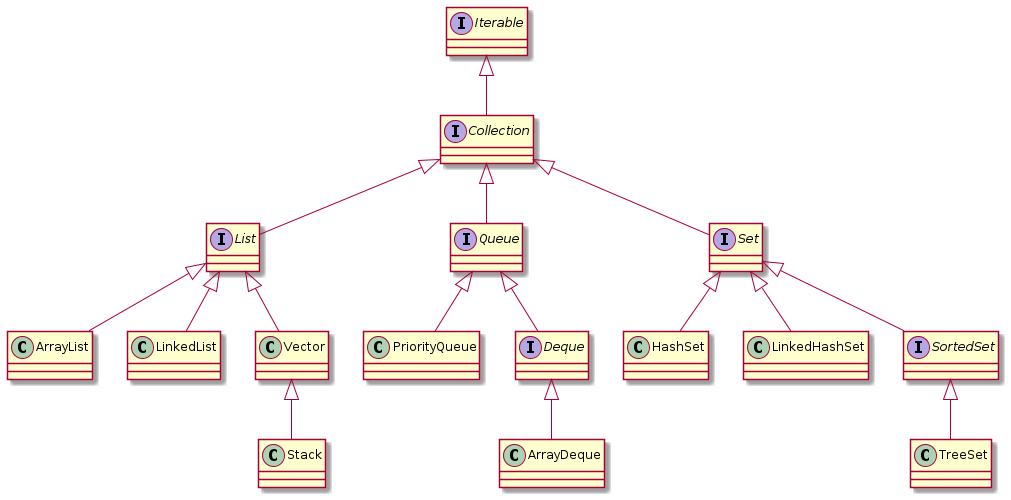
\includegraphics[width=\textwidth]{07_collection/collection.png}
\end{frame}


\subsection{List}

\begin{frame}[fragile]{List}
	A list is an ordered collection.
	\vfill
	The implementation \texttt{LinkedList} is a double-linked list.
	\begin{lstlisting}[basicstyle=\ttfamily\scriptsize]
	public static void main(String[] args) {
	
	    List<String> list = new LinkedList<String>();
	    
	    list.add("foo"); 
	    list.add("foo"); // insert "foo" at the end
	    list.add("bar");
	    list.add("foo");
	    list.remove("foo"); // removes the first "foo"
	    
	    System.out.println(list); // prints: [foo, bar, foo]
	}
	\end{lstlisting}
\url{https://docs.oracle.com/en/java/javase/11/docs/api/java.base/java/util/List.html}
\end{frame}
	
\begin{frame}[fragile]{List Methods}
	some useful List methods:\\
	\vspace{1em}
	\begin{tabular}{ r l r }
		void & \texttt{add(int index, E element)}
		& \footnotesize{insert element at position index} \\
		E &\texttt{get(int index)}
		& \footnotesize{get element at position index} \\
		E &\texttt{set(int index, E element)}
		& \footnotesize{replace element at position index} \\
		E &\texttt{remove(int index)}
		& \footnotesize{remove element at position index}
	\end{tabular}
	\vfill
	some useful LinkedList methods:\\
	\vspace{1em}
	\begin{tabular}{ r l r }
		void & \texttt{addFirst(E element)}
		& \footnotesize{append element to the beginning} \\
		E & \texttt{getFirst()}
		& \footnotesize{get first element} \\
		void & \texttt{addLast(E element)}
		& \footnotesize{append element to the end} \\
		E & \texttt{getLast()}
		& \footnotesize{get last element}
	\end{tabular}
\end{frame}

\begin{frame}[allowframebreaks]{LinkedList vs ArrayList}
	
	ArrayList\footnote{ \url{https://docs.oracle.com/en/java/javase/11/docs/api/java.base/java/util/ArrayList.html}}:
	\begin{itemize}
		\item Resizeable-array implementation
		\item List has a specific capacity, may have to be resized (automatically)
		\item But \texttt{add()} runs in amortized constant time (O(n))
		\item \texttt{size}, \texttt{isEmpty}, \texttt{get}, \texttt{set}, \texttt{iterator}, and \texttt{listIterator} in constant time
		\item Any other method runs in linear time
	\end{itemize}

	\framebreak
	LinkedList\footnote{\url{https://docs.oracle.com/en/java/javase/11/docs/api/java.base/java/util/LinkedList.html}}:
	\begin{itemize}
		\item Doubly-linked list implementation
		\item Can grow indefinitely without resizing (memory constraint)
		\item \texttt{add}, \texttt{get} and \texttt{remove} at the end/beginning fast
		\item Any other element, time depending on position
	\end{itemize}
	 

\end{frame}

\subsection{Iterating}
\begin{frame}[fragile]{For Loop}
	The for loop can iterate over every element of a collection:\\
	\hspace{1em}\texttt{for (E e : collection)}
	\begin{lstlisting}
	public static void main(String[] args) {
	
	    List<Integer> list = 
	        new LinkedList<Integer>();
	    
	    list.add(1);
	    list.add(3);
	    list.add(3);
	    list.add(7);
	    
	    for (Integer i : list) {
	        System.out.print(i + " "); // prints: 1 3 3 7
	    }
	}
	\end{lstlisting}
\end{frame}

\begin{frame}[fragile]{Iterator}
	An iterator iterates step by step over a collection.
	\begin{lstlisting}[basicstyle=\ttfamily\scriptsize]
	public static void main(String[] args) {
	
	    List<Integer> list = new LinkedList<Integer>();
	    
	    list.add(1);
	    list.add(3);
	    list.add(3);
	    list.add(7);
	    
	    Iterator<Integer> iter = list.iterator();
	    
	    while (iter.hasNext()) {
	        System.out.print(iter.next());
	    }
	    // prints: 1337
	}
	\end{lstlisting}
\end{frame}

\begin{frame}[fragile]{Iterator}
	A standard iterator has only three methods:
	\begin{itemize}
	\item \texttt{boolean hasNext()} - indicates if therer are more elements
	\item \texttt{E next()} - returns the next element
	\item \texttt{void remove()} - returns the current element
	\end{itemize}
	\vspace{1em}
	The iterator is instanced via \texttt{collection.iterator()} :
	\begin{lstlisting}[basicstyle=\ttfamily\scriptsize]
	    Collection<E> collection = new Implementation<E>;
	    Iterator<E> iter = collection.iterator();
	\end{lstlisting}
	Special iterators like \emph{ListIterator} are more sophisticated.
\end{frame}

\section{Hands-On}
\begin{frame}[fragile]{Library (Part 1)}
	
	\begin{center}
		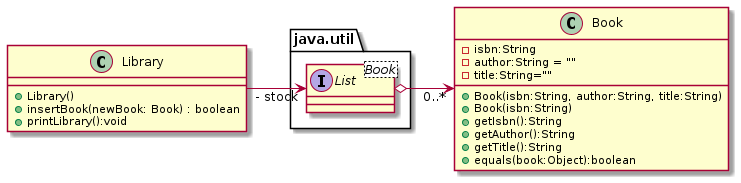
\includegraphics[width=\textwidth]{07_collection/hands_on_01.png}
	\end{center}

	
\end{frame}
\subsection{Comparable}
\begin{frame}{Comparable}
	content...
\end{frame}
\begin{frame}{Part 2}

		\begin{center}
		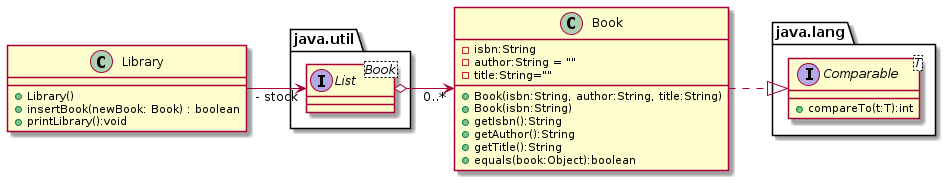
\includegraphics[width=\textwidth]{07_collection/hands_on_02.png}
		\end{center}

\end{frame}
\subsection{Collections}
\begin{frame}{Collections}
	content...
\end{frame}
\begin{frame}{Part 3}

	\begin{center}
		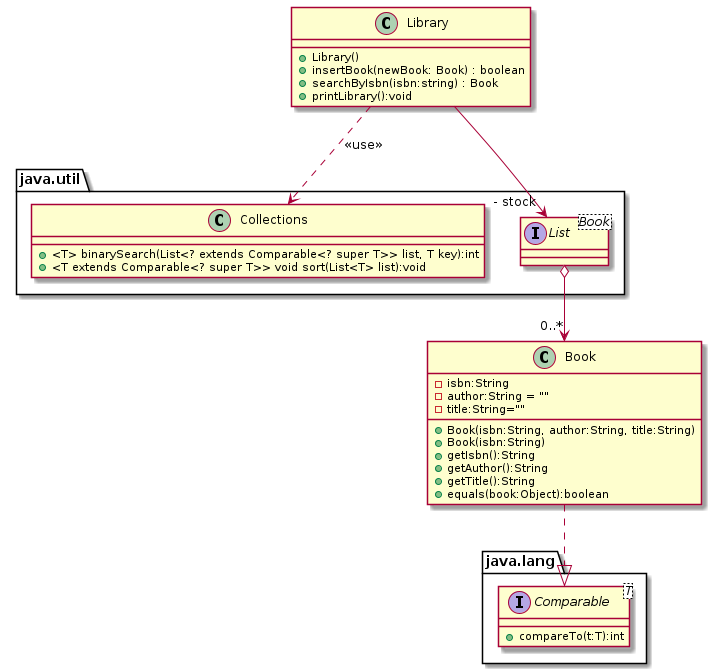
\includegraphics[scale=.34]{07_collection/hands_on_03.png}
	\end{center}

\end{frame}

\begin{frame}{Part 4}

	\begin{center}
		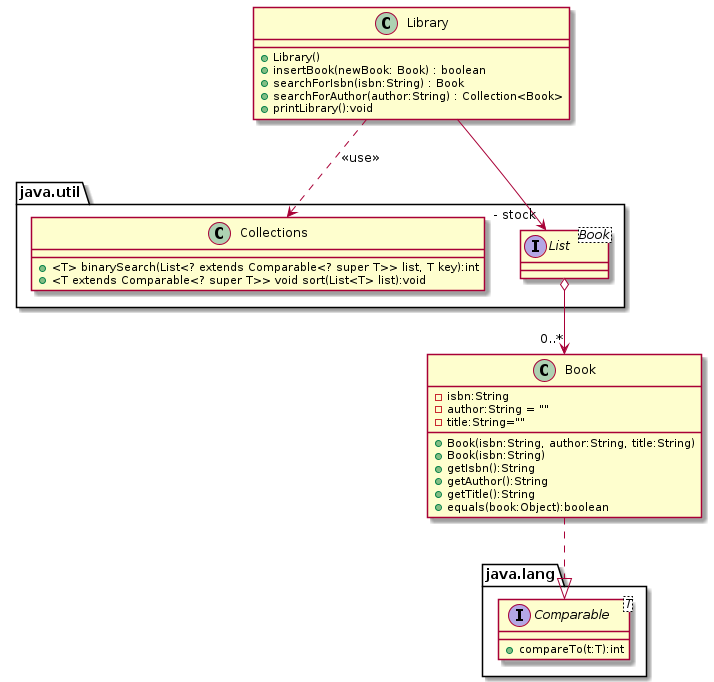
\includegraphics[scale=.34]{07_collection/hands_on_04.png}
	\end{center}
		

		
\end{frame}


\end{document}